\chapter{生物信息学与序列分析}\label{ch:b3:bioinformatics}

一位生物学家刚从一种深海蠕虫中测得一个基因，
便将其 \num{300} 个氨基酸输入网页表单，三秒后
便得知该蛋白质是一种人类激酶的远亲，
与之在 \num{280} 个残基上具有 \qty{31}{\%} 的同一性，
而这一相似性纯属偶然的概率为 $10^{-40}$。三秒钟的背后是
一种 1970 年提出的\omterm{thm:b3:bioinformatics:nw}{动态规划}算法、一套随机\omterm{def:b3:bioinformatics:alignment}{比对}的统计理论，
以及从数千个蛋白质家族中提炼出的\omterm{def:b3:bioinformatics:matrices}{替换矩阵}，
还有一个含约千亿个残基的数据库。
本章讨论的是这个“黑箱”内部的推理：两条序列如何\omterm{def:b3:bioinformatics:alignment}{比对}，
才能被证明是最优的，得分如何
才具有意义，如何区分真正的匹配与偶然的巧合，
以及如何在一个此前无人研究过的
基因组中发现模式。数学并不复杂——涉及递推关系、对数和
泊松分布——但值得掌握，因为
从序列比较得出的每一个结论都依赖于它。

\section{两条序列的比对}

\begin{definition}[比对与得分]\label{def:b3:bioinformatics:alignment}
\index{序列比对}\index{空位罚分}\index{全局比对}\index{局部比对}
两条序列的\emph{比对}是指将二者上下排列，
在其中插入\emph{空位}（--），使每一列配对的是一个残基与一个残基，或一个残基与一个空位，
且任何一列都不允许两个空位相配。其
\emph{得分}为各列之和：每对残基计入替换得分 $s(a,b)$，
每个空位计入一项\emph{空位罚分}。空位罚分可取线性形式，
即每个空位位置计 $-d$；更符合实际的是
\emph{仿射}罚分 $-d - (k-1)e$，用于连续 $k$ 个空位的一段，
其中开空位代价 $d$ 大于延伸代价 $e$，因为一次
插入若干残基在进化上只是一次事件。
\emph{全局}比对覆盖两条序列的全长；一个\emph{局部}
比对则寻找得分最高的一对子串，并忽略其余部分，
这正是人们所需要的——当一个共同的结构域
位于两个其他方面无关的蛋白质中时。
\end{definition}

\begin{theorem}[尼德曼–翁施]\label{thm:b3:bioinformatics:nw}
\index{尼德曼–翁施}\index{动态规划}\index{史密斯–沃特曼}
设 $x = x_{1}\dots x_{m}$ 与 $y = y_{1}\dots y_{n}$，线性\omterm{def:b3:bioinformatics:alignment}{空位罚分}为
$d$。定义 $F(i,j)$ 为
前缀 $x_{1}\dots x_{i}$ 与 $y_{1}\dots y_{j}$ 的最优\omterm{def:b3:bioinformatics:alignment}{全局比对}得分。则
$F(i,0) = -id$，$F(0,j) = -jd$，且对 $i,j \ge 1$，
\[
F(i,j) = \max\bigl\{\,F(i-1,j-1) + s(x_{i},y_{j}),\;
F(i-1,j) - d,\; F(i,j-1) - d\,\bigr\}.
\]
$F(m,n)$ 为最优全局得分，最优\omterm{def:b3:bioinformatics:alignment}{比对}可
通过从 $(m,n)$ 出发\omterm{met:b3:bioinformatics:align}{回溯}，取出产生各个最大值的选择而得到，
整个计算需要 $mn$ 步。\omterm{def:b3:bioinformatics:alignment}{局部比对}的
\emph{\omterm{thm:b3:bioinformatics:nw}{史密斯–沃特曼}}变体在取最大值时加入 $0$ 作为第四个选项，
将边界置为 $0$，并在表中
最大的元素处读取结果。
\end{theorem}
\begin{proof}
考虑两个前缀的任一\omterm{def:b3:bioinformatics:alignment}{比对}的最后一列，它只能是
三种情形之一：$x_{i}$ 对 $y_{j}$、$x_{i}$ 对空位，或空位对
$y_{j}$。去掉该列后，分别得到 $(x_{1}\dots x_{i-1},
y_{1}\dots y_{j-1})$、$(x_{1}\dots x_{i-1}, y_{1}\dots y_{j})$ 或
$(x_{1}\dots x_{i}, y_{1}\dots y_{j-1})$ 的\omterm{def:b3:bioinformatics:alignment}{比对}，其得分至多为该前缀对的
$F$ 值；反之，这些最优\omterm{def:b3:bioinformatics:alignment}{比对}中的每一个
都可通过添加对应的最后一列而延伸。因此，以各类列结尾的最佳得分
等于较短前缀对的 $F$ 值加上该列的得分，
而最优值为三者中的最大值。
边界值是唯一确定的（与空前缀配对时只可能出现空位）。
对 $i + j$ 作归纳即可填满整张表；格子数为 $(m+1)(n+1)$。
对\omterm{def:b3:bioinformatics:alignment}{局部比对}，多出的选项 $0$ 表示“在此处开始
新的\omterm{def:b3:bioinformatics:alignment}{比对}”，这使得 $F(i,j)$ 为\emph{结束于}
$(i,j)$ 的\omterm{def:b3:bioinformatics:alignment}{比对}的最优得分，而最优\omterm{def:b3:bioinformatics:alignment}{局部比对}结束于某处。
\end{proof}

\begin{example}[一张四乘三的表]\label{ex:b3:bioinformatics:nw-example}
将 GAT 与 GCAT \omterm{def:b3:bioinformatics:alignment}{比对}，匹配计 $+1$，错配计 $-1$，
$d = 1$。顶行边界为 $0, -1, -2, -3, -4$，侧边界为 $0, -1,
-2, -3$。逐行填表：$F(\text{G},\text{G}) = 1$，
$F(\text{G},\text{C}) = 0$，$F(\text{G},\text{A}) = -1$，
$F(\text{G},\text{T}) = -2$；$F(\text{A},\text{G}) = 0$，
$F(\text{A},\text{C}) = 0$，$F(\text{A},\text{A}) = 1$，
$F(\text{A},\text{T}) = 0$；$F(\text{T},\text{G}) = -1$，
$F(\text{T},\text{C}) = -1$，$F(\text{T},\text{A}) = 0$，
$F(\text{T},\text{T}) = 2$。最优值为 $2$，\omterm{met:b3:bioinformatics:align}{回溯}
——从 (T,T) 沿对角线，从 (A,A) 沿对角线，再从 (G,C) 向左至
(G,G)，再沿对角线——得到
\[
\begin{array}{c}
\texttt{G-AT}\\
\texttt{GCAT}
\end{array}
\]
三个匹配、一个空位：$3 - 1 = 2$。
\end{example}

\begin{omfigure}
\begin{tikzpicture}[every node/.style={font=\small}, >=stealth]
  \def\dx{1.0}\def\dy{0.8}
  % headers
  \foreach \j/\c in {1/G,2/C,3/A,4/T} \node[omDef, font=\small\bfseries] at (\j*\dx+0.5,0.4) {\c};
  \foreach \i/\c in {1/G,2/A,3/T} \node[omDef, font=\small\bfseries] at (-0.5,-\i*\dy-0.4) {\c};
  % grid
  \draw[gray!60] (0,0) grid[xstep=\dx, ystep=\dy] (5*\dx,-4*\dy);
  % values
  \foreach \i/\j/\v in {0/0/0,0/1/-1,0/2/-2,0/3/-3,0/4/-4,1/0/-1,2/0/-2,3/0/-3, 1/1/1,1/2/0,1/3/-1,1/4/-2, 2/1/0,2/2/0,2/3/1,2/4/0, 3/1/-1,3/2/-1,3/3/0,3/4/2}
    \node at (\j*\dx+0.5,-\i*\dy-0.4) {$\v$};
  % traceback path highlighted
  \foreach \i/\j in {0/0,1/1,1/2,2/3,3/4} \draw[omThm, very thick] (\j*\dx+0.05,-\i*\dy-0.05) rectangle (\j*\dx+\dx-0.05,-\i*\dy-\dy+0.05);
  \draw[->, omThm, very thick, shorten >=8pt, shorten <=8pt] (4.5,-2.8) -- (3.5,-2.0);
  \draw[->, omThm, very thick, shorten >=8pt, shorten <=8pt] (3.5,-2.0) -- (2.5,-1.2);
  \draw[->, omThm, very thick, shorten >=8pt, shorten <=8pt] (2.5,-1.2) -- (1.5,-1.2);
  \draw[->, omThm, very thick, shorten >=8pt, shorten <=8pt] (1.5,-1.2) -- (0.5,-0.4);
  \node[right, align=left] at (5.6,-1.6) {回溯自 $F(3,4) = 2$：\\对角线，对角线，\\左移（GAT 中的空位），对角线 \\[3pt] \texttt{G-AT}\\\texttt{GCAT}};
\end{tikzpicture}

{\small 针对 GAT 与 GCAT 的 Needleman--Wunsch 表（匹配 $+1$，
错配 $-1$，空位 $-1$）。每个单元格记录以该处结尾的两个
前缀的最佳得分；自右下角\omterm{met:b3:bioinformatics:align}{回溯}所得的红色路径即为
最优\omterm{def:b3:bioinformatics:alignment}{比对}。}
\end{omfigure}

\begin{method}[两条序列的比对]\label{met:b3:bioinformatics:align}
\index{回溯}
（1）选择打分方案：根据预期的
分化程度选取\omterm{def:b3:bioinformatics:matrices}{替换矩阵}（距离未知的蛋白质用 BLOSUM62；
DNA 用匹配/错配），以及仿射\omterm{def:b3:bioinformatics:alignment}{空位罚分}（通常取开启罚分 $-11$、延伸罚分 $-1$，
配合 BLOSUM62 使用）。（2）决定全局还是局部：两条序列若被认为
在整个长度上同源，则用\omterm{def:b3:bioinformatics:alignment}{全局比对}，否则用\omterm{def:b3:bioinformatics:alignment}{局部比对}。
（3）按递推式填写表格，为每个单元格保存一个指针，
指向取得最大值的选择。（4）自 $(m,n)$ 起\omterm{met:b3:bioinformatics:align}{回溯}
（\omterm{def:b3:bioinformatics:alignment}{全局比对}）；或自最大值单元格\omterm{met:b3:bioinformatics:align}{回溯}至零（\omterm{def:b3:bioinformatics:alignment}{局部比对}），
由右至左写出\omterm{def:b3:bioinformatics:alignment}{比对}。（5）评判结果时，不看其原始
得分，而看其统计显著性（见下文），并检查\omterm{def:b3:bioinformatics:alignment}{比对}本身：
过长的空位、低复杂度片段以及仅限于重复序列内的\omterm{def:b3:bioinformatics:alignment}{比对}，都是
警示信号。
\end{method}

\section{打分：一次匹配值多少}

\begin{definition}[替换矩阵]\label{def:b3:bioinformatics:matrices}
\index{替换矩阵}\index{BLOSUM}\index{PAM}\index{对数几率得分}
称\emph{替换矩阵}为以\emph{对数几率得分}形式给出每对氨基酸
$s(a,b)$ 的矩阵：
\[
s(a,b) = \frac{1}{\lambda}\,\log\frac{q_{ab}}{p_{a}\,p_{b}},
\]
其中 $q_{ab}$ 为在相关蛋白质的可信\omterm{def:b3:bioinformatics:alignment}{比对}中 $a$ 与 $b$ 被
对齐的频率，$p_{a} p_{b}$ 为
二者随机配对的频率，且 $\lambda$ 为
一个选定的标度，使各项取值为便于使用的整数。正得分
表示该对在同源序列中出现的频率高于随机情形；
同一性得分在稀有氨基酸上最大（BLOSUM62 中色氨酸 $+11$，
半胱氨酸 $+9$），在常见氨基酸上最小（亮氨酸 $+4$，
丙氨酸 $+4$），保守替换（异亮氨酸–缬氨酸 $+3$）
得正分，而非保守替换（色氨酸–甘氨酸 $-2$）
得负分。\emph{PAM} 矩阵（戴霍夫，1978）由
亲缘关系较近的蛋白质推导而来，并通过矩阵乘法
外推至更远的距离；\emph{BLOSUM} 矩阵（亨尼科夫与亨尼科夫，1992）
则是直接在按给定同一性聚类的\omterm{def:b3:bioinformatics:alignment}{比对}序列块中统计得到的
——BLOSUM62 取自同一性为 \qty{62}{\%} 的序列块——
并因为它们是在实际使用的距离上经实测、而非外推得到，
故成为默认选择。
\end{definition}

\begin{proposition}[为何采用对数几率]\label{prop:b3:bioinformatics:logodds}
\index{期望得分}
对于用于\omterm{def:b3:bioinformatics:alignment}{局部比对}的打分方案，随机配对列的\omterm{prop:b3:bioinformatics:logodds}{期望得分}
$\sum_{a,b} p_{a} p_{b}\, s(a,b)$ 必须为
负，且须有部分得分为正；否则随机\omterm{def:b3:bioinformatics:alignment}{比对}会无限增长，
使得分最高的片段
将是整条序列。在此条件下，任何此类方案
都等价于对\emph{某些}目标频率的对数几率方案，
其目标频率为 $q_{ab}$——它所找到的最优\omterm{def:b3:bioinformatics:alignment}{比对}，是
残基对分布与 $q_{ab}$ 一致的\omterm{def:b3:bioinformatics:alignment}{比对}。因此，选择矩阵
即是选择所期望检测的分化程度：适用于近缘关系的
矩阵（BLOSUM80、PAM30）正分更尖锐、负分更严厉；适用于远缘关系的
矩阵（BLOSUM45、PAM250）则更为平缓。
\end{proposition}
\admitted

\begin{example}[同一性、相似性与暮光区]\label{ex:b3:bioinformatics:twilight}
两条随机蛋白质序列经带空位的最优\omterm{def:b3:bioinformatics:alignment}{比对}，偶然可达到约
\qtyrange{15}{20}{\%} 的同一性。高于 \qty{35}{\%} 的同一性
且覆盖百余个残基时，两条蛋白质几乎肯定同源；
介于 \qty{20}{\%} 与 \qty{35}{\%} 之间的区间为\emph{暮光区}，
仅凭同一性无法判定，须借助下文的统计量。
同源蛋白也可远低于该区间：血红蛋白与肌红蛋白的
亚基的同一性为 \qty{25}{\%}，溶菌酶与 $\alpha$-乳白蛋白
的同一性为 \qty{40}{\%}，而许多具有相同折叠类型的蛋白质对
同一性不足 \qty{15}{\%}，只有比较谱或结构才能检出。
\end{example}

\section{在数据库中搜索}

\begin{definition}[BLAST]\label{def:b3:bioinformatics:blast}
\index{BLAST}\index{种子}\index{高分片段对}
若用完整\omterm{thm:b3:bioinformatics:nw}{动态规划}将含 \num{300} 个残基的查询序列
与含 $10^{11}$ 个残基的数据库\omterm{def:b3:bioinformatics:alignment}{比对}，每次搜索需要 $3\times 10^{13}$ 次单元格更新。
\emph{BLAST}（阿尔特舒尔等人，1990）以三个步骤略微牺牲灵敏度，
换取约千倍的速度：（1）列出查询序列的
\emph{词}（蛋白质取三个残基，DNA 取十一个
碱基）及其高分近邻；（2）在数据库中扫描精确词匹配，
即\emph{种子}；（3）将每个种子向两个方向无空位延伸，
直至得分较其最佳值下降一设定量，
保留\emph{高分片段对}（HSP），随后以
窄带中带空位的\omterm{thm:b3:bioinformatics:nw}{动态规划}连接相邻的 HSP。真正的
同源序列几乎总与之共有至少一个精确的三残基词；
偶然的相似则很少如此，且从不被
延伸。
\end{definition}

\begin{omfigure}
\begin{tikzpicture}[every node/.style={font=\scriptsize}, >=stealth]
  % query and database sequences as bars
  \draw[very thick, omDef] (0,2.0) -- (5,2.0); \node[left] at (-0.1,2.0) {查询序列};
  \draw[very thick, gray] (0,0.6) -- (11,0.6); \node[left] at (-0.1,0.6) {数据库};
  % seeds
  \foreach \q/\d in {1.2/3.6, 2.8/5.2, 4.1/9.3} {
    \fill[omThm] (\q-0.15,1.9) rectangle (\q+0.15,2.1);
    \fill[omThm] (\d-0.15,0.5) rectangle (\d+0.15,0.7);
    \draw[omThm, thick] (\q,1.85) -- (\d,0.75);
  }
  \node[above] at (1.2,2.15) {词}; \node[above] at (2.8,2.15) {词}; \node[above] at (4.1,2.15) {词};
  % extension of the first two (same diagonal) -> HSP
  \draw[<->, very thick, omMeth!70!black] (2.6,0.3) -- (6.2,0.3); \node[below] at (4.4,0.25) {无空位延伸：一个 HSP};
  % third seed: extension fails
  \draw[omProp, thick, dashed] (8.8,0.3) -- (9.8,0.3); \node[below, omProp] at (9.3,0.25) {得分下降：舍弃};
  \node[right, align=left] at (5.5,2.0) {1. 查询序列的词 \\2. 数据库中的精确命中（种子）\\3. 延伸，保留高分对};
\end{tikzpicture}

{\small \omterm{def:b3:bioinformatics:blast}{BLAST} 启发式算法。查询序列与
数据库条目共有的短精确词（红色）为\omterm{def:b3:bioinformatics:blast}{种子}；每个\omterm{def:b3:bioinformatics:blast}{种子}沿其对角线延伸，
只要得分持续上升，并且只有保持高分的延伸才成为
\omterm{def:b3:bioinformatics:blast}{高分片段对}。}
\end{omfigure}

\begin{theorem}[随机命中的统计]\label{thm:b3:bioinformatics:evalue}
\index{E 值}\index{比特得分}\index{Karlin--Altschul}
设查询序列长度为 $m$，在总长度为
$n$ 的数据库中搜索，所用计分方案的\omterm{prop:b3:bioinformatics:logodds}{期望得分}为负。则偶然出现的、
得分至少为 $S$ 的无空位\omterm{def:b3:bioinformatics:alignment}{局部比对}数
服从均值为下式的泊松分布：
\[
E = K\,m\,n\,e^{-\lambda S},
\]
其中 $\lambda$ 与 $K$ 仅依赖于计分方案和
残基频率（$\lambda$ 为对数几率矩阵的尺度）。
$E$ 称为得分 $S$ 的\emph{期望值}。将得分写成
\emph{比特}形式，$S' = (\lambda S - \ln K)/\ln 2$，公式化为
$E = m n\, 2^{-S'}$，而至少有一次偶然\omterm{def:b3:bioinformatics:alignment}{比对}
达到 $S$ 的概率为 $P = 1 - e^{-E}$，当 $E$
很小时，它等于 $E$。
\end{theorem}
\begin{proof}[部分证明]
指数尾部即 \omterm{thm:b3:bioinformatics:evalue}{Karlin--Altschul} 定理，在本阶段不加证明地承认：
负漂移随机游走的最大片段得分，其分布的尾部
以 $e^{-\lambda S}$ 衰减，其中 $\lambda$ 为
方程 $\sum_{a,b} p_{a} p_{b} e^{\lambda s(a,b)} = 1$ 的正根——
这恰好是使对数几率矩阵自洽的方程。
有了这一尾部，其余便是计数。高分片段可以从
$mn$ 对位置中的任一对开始，它们稀少，且
近似独立；因此超过 $S$ 的此类片段数服从
均值与 $mn$ 及尾部概率成正比的泊松分布，
$E = Kmn\,e^{-\lambda S}$。无一出现的概率为 $e^{-E}$。
\omterm{thm:b3:bioinformatics:evalue}{比特得分}的替换只是代数运算：$e^{-\lambda S} K = 2^{-(\lambda S -
\ln K)/\ln 2}$。对于有空位\omterm{def:b3:bioinformatics:alignment}{比对}，同样的形式成立，其中 $\lambda$
与 $K$ 通过模拟估计。
\end{proof}

\begin{example}[读取 E 值]\label{ex:b3:bioinformatics:evalue}
一条长为 \num{250} 个残基的查询序列，搜索长为 $5\times 10^{10}$
个残基的数据库，有 $mn = 1.25\times 10^{13} \approx 2^{43.5}$。
\omterm{thm:b3:bioinformatics:evalue}{比特得分}为 $60$ 的命中有 $E = 2^{43.5 - 60} = 2^{-16.5} \approx 10^{-5}$：
几乎可以肯定是同源物。$S' = 40$ 的命中有 $E = 2^{3.5}
\approx 11$：偶然可期望出现十一次这样的得分，
该命中毫无意义。\emph{同一}\omterm{def:b3:bioinformatics:alignment}{比对}、相同的\omterm{thm:b3:bioinformatics:evalue}{比特得分}，
若在大十倍的数据库中搜索，其 $E$ 也
增大十倍——显著性是搜索的属性，而非配对的属性。
通常采用的阈值为：$E < 10^{-3}$ 时可有把握地认为是同源物；
$E \approx 0.01$--$1$ 则值得用谱方法再次检查。
\end{example}

\begin{omfigure}
\begin{tikzpicture}
\begin{axis}[
  width=0.7\linewidth, height=5.6cm,
  axis x line=bottom, axis y line=left,
  xmin=25, xmax=70, ymin=0.000000001, ymax=100000000, ymode=log,
  xlabel={比特得分 $S'$}, ylabel={$E$},
  xlabel style={font=\small, at={(axis description cs:0.5,-0.12)}, anchor=north},
  ylabel style={font=\small},
  tick label style={font=\small}, xtick={30,40,50,60,70},
  clip=false,
]
\addplot[very thick, omDef, domain=25:70, samples=2] {2^(43.5-x)};
\addplot[very thick, omThm, domain=25:70, samples=2] {2^(46.8-x)};
\addplot[dashed, gray, domain=25:70, samples=2] {0.001};
\node[font=\scriptsize, gray, anchor=south west] at (axis cs:25.5,0.0012) {$E = 10^{-3}$};
\node[font=\scriptsize, omDef, anchor=north west] at (axis cs:26,0.00002) {$mn = 1.25\times 10^{13}$};
\node[font=\scriptsize, omThm, anchor=south west] at (axis cs:45,30) {$mn$ 大十倍};
\end{axis}
\end{tikzpicture}

{\small $E = mn\,2^{-S'}$：每增加一个比特，偶然命中的期望数减半；
数据库大十倍，同一\omterm{def:b3:bioinformatics:alignment}{比对}的显著性
下降 $3.3$ 个比特。}
\end{omfigure}

\section{谱、隐状态与基序}

\begin{definition}[多序列比对与谱]\label{def:b3:bioinformatics:msa}
\index{多序列比对}\index{谱}\index{谱隐马尔可夫模型}
\emph{多\omterm{def:b3:bioinformatics:alignment}{序列比对}}将一族序列排列为
同源残基的列。对 $k$ 条序列的精确\omterm{thm:b3:bioinformatics:nw}{动态规划}
代价为 $n^{k}$，超过三条即不可行；实用程序
采用\emph{渐进地}\omterm{def:b3:bioinformatics:alignment}{比对}：先由引导树找出最接近的一对，
再将序列与类群逐一\omterm{def:b3:bioinformatics:alignment}{比对}到不断增长的\omterm{def:b3:bioinformatics:alignment}{比对}结果上，并进行若干轮
修正。完成的\omterm{def:b3:bioinformatics:alignment}{比对}可概括为一个\emph{谱}：
对每一列，给出各残基及空位的频率。一个
\emph{谱隐马尔可夫模型}将其形式化为一条匹配状态链，
每个保守列对应一个状态，各状态以各自的概率发射残基；
插入状态与删除状态允许每个位置多出或缺失残基。
某一家族（即 Pfam 条目）的模型，
以状态路径上最佳路径的概率为新序列打分，
能够找出远低于两两比较“暮光区”的同源物，
因为只耐受疏水残基的列能够说明这一点，
而单条序列则不能。
\end{definition}

\begin{omfigure}
\begin{tikzpicture}[every node/.style={font=\scriptsize}, >=stealth]
  % match states
  \foreach \i in {1,2,3,4} { \draw[thick, fill=omDef!25] (2.2*\i-0.5,0) rectangle (2.2*\i+0.5,0.7); \node at (2.2*\i,0.35) {M$_{\i}$}; }
  % insert states (diamonds) above
  \foreach \i in {1,2,3} { \draw[thick, fill=omProp!30] (2.2*\i+1.1,1.6) -- (2.2*\i+1.55,2.05) -- (2.2*\i+1.1,2.5) -- (2.2*\i+0.65,2.05) -- cycle; \node at (2.2*\i+1.1,2.05) {I$_{\i}$}; }
  % delete states (circles) below
  \foreach \i in {2,3} { \draw[thick, fill=gray!20] (2.2*\i,-1.3) circle (0.4); \node at (2.2*\i,-1.3) {D$_{\i}$}; }
  % transitions match->match
  \foreach \i in {1,2,3} \draw[->, thick] (2.2*\i+0.5,0.35) -- (2.2*\i+1.7,0.35);
  % match->insert->match
  \foreach \i in {1,2,3} { \draw[->, thick, omProp] (2.2*\i+0.3,0.7) -- (2.2*\i+0.9,1.65); \draw[->, thick, omProp] (2.2*\i+1.3,1.65) -- (2.2*\i+1.9,0.7); \draw[->, thick, omProp] (2.2*\i+1.1,2.5) arc[start angle=200, end angle=-20, radius=0.3]; }
  % match->delete->match
  \draw[->, thick, gray] (2.2+0.3,0) -- (4.4-0.3,-1.0); \draw[->, thick, gray] (4.4+0.3,-1.0) -- (6.6-0.3,0); \draw[->, thick, gray] (4.4+0.4,-1.3) -- (6.6-0.4,-1.3); \draw[->, thick, gray] (6.6+0.3,-1.0) -- (8.8-0.3,0);
  \node[below, align=center] at (2.2,-1.2) {发射：每个匹配状态一个残基 \\分布};
  \node[right, align=left] at (9.6,1.2) {序列依其 \\最佳路径打分：匹配、\\插入（橙色）和 \\删除（灰色）};
\end{tikzpicture}

{\small 一个四列家族的\omterm{def:b3:bioinformatics:msa}{谱隐马尔可夫模型}。每
个匹配状态 M 以该列自身的频率发射一个残基；
插入状态 I（带自环）允许额外残基插入，删除状态 D
跳过一列。给序列打分即求其最可能路径。}
\end{omfigure}

\begin{definition}[基序与信息量]\label{def:b3:bioinformatics:motif}
\index{基序}\index{位置权重矩阵}\index{信息量}\index{序列标识图}
\emph{基序}是一段短模式——转录因子结合位点、
剪接信号、磷酸化位点——由\emph{位置权重矩阵}表示，
其元素为频率 $f_{i}(b)$，即每个碱基或残基 $b$
在每个位置 $i$ 上的频率。位置 $i$ 的\emph{信息量}
为 $R_{i} = 2 - H_{i}$ 比特（对 DNA 而言），其中 $H_{i} =
-\sum_{b} f_{i}(b)\log_{2} f_{i}(b)$ 为该位置的熵：不变碱基的信息量为 $2$ 比特，
四种碱基等可能出现的位置，信息量为 $0$。
总信息量 $R = \sum_{i} R_{i}$ 以\emph{序列标识图}表示，每个
位置为一叠字母，其总高度为 $R_{i}$，字母大小
按频率确定。
\end{definition}

\begin{proposition}[一个位点需要多少信息]\label{prop:b3:bioinformatics:bits}
\index{信息量!与基因组大小}
某位点须在基因组中恰好出现 $\gamma$ 次、别处不再出现，该基因组共 $G$ 个位置，
则所需\omterm{def:b3:bioinformatics:motif}{信息量}约为 $R_{\text{所需}} = \log_{2}(G/\gamma)$
比特：\omterm{def:b3:bioinformatics:motif}{基序}须把 $G$ 个候选位置
缩减为 $\gamma$ 个真实位置，每一比特使候选数减半。
研究充分的细菌调控因子的已观察\omterm{def:b3:bioinformatics:motif}{基序}与此预测相符——
\emph{E.~coli} 中阻遏蛋白结合几十处位点的情形，
在 \qty{4.6}{Mb} 基因组中，其位点携带 \numrange{16}{18} 比特；
真核转录因子\omterm{def:b3:bioinformatics:motif}{基序}仅携带 \numrange{8}{12} 比特，
在 $3\times 10^{9}$ 的基因组中，单靠它们无法确定靶点，
这正是它们需以组合方式发挥作用、并依托
在\cref{ch:b3:chromatin-epigenetics}中所述的开放\omterm{def:b3:chromatin-epigenetics:nucleosome}{染色质}。
\end{proposition}
\begin{proof}
随机位置与\omterm{def:b3:bioinformatics:motif}{信息量}为 $R$ 的\omterm{def:b3:bioinformatics:motif}{基序}匹配的概率约为
$2^{-R}$（每一比特的特异性使机会减半），
因此在 $G$ 个位置中偶然匹配的期望次数为 $G\,2^{-R}$。
要使真实位点突显出来，此数应为 $\gamma$ 量级或更小：
$G\,2^{-R} \le \gamma$，即 $R \ge \log_{2}(G/\gamma)$。
\end{proof}

\begin{example}[期望的偶然匹配数]\label{ex:b3:bioinformatics:motif-numbers}
一个由六个固定碱基组成的限制性位点，其 $R = 12$ 比特，与随机位置匹配的概率为
$4^{-6} = 2^{-12}$，约 \num{1100} 次
出现于 \emph{E.~coli} 的 \qty{4.6}{Mb} 基因组中（双链均读取，
该位点为回文序列，故每个位置只计一次），在人类基因组中出现 $7\times 10^{5}$
次。一个真核因子的\omterm{def:b3:bioinformatics:motif}{基序}携带
$10$ 比特信息，在人类基因组中的匹配数为 $3\times 10^{9}\times 2^{-10} \approx 3$
即约 300 万个位置，远多于它所调控的
基因，多出数千倍。单独一个\omterm{def:b3:bioinformatics:motif}{基序}在大型基因组中
是较弱的预测指标；真正使预测成立的是\omterm{def:b3:chromatin-epigenetics:nucleosome}{染色质}状态、相邻\omterm{def:b3:bioinformatics:motif}{基序}和
该位点在物种间的保守性。
\end{example}

\begin{omfigure}
\begin{tikzpicture}[every node/.style={font=\scriptsize}]
  % sequence logo: TATA box-like 8 positions, stack heights = information content (1 bit = 1 cm)
  \draw[->] (0,0) -- (0,2.2); \node[left] at (-0.05,2.0) {2}; \node[left] at (-0.05,1.0) {1}; \node[left] at (-0.05,0) {0}; \node[rotate=90, above] at (-0.55,1.1) {比特};
  \draw (0,0) -- (8.6,0);
  \node[anchor=south, inner sep=0] at (0.5,0) {\resizebox{0.6cm}{1.9cm}{\textcolor{omThm}{\bfseries T}}};
  \node[anchor=south, inner sep=0] at (1.5,0) {\resizebox{0.6cm}{1.9cm}{\textcolor{omMeth!70!black}{\bfseries A}}};
  \node[anchor=south, inner sep=0] at (2.5,0) {\resizebox{0.6cm}{1.7cm}{\textcolor{omThm}{\bfseries T}}};
  \node[anchor=south, inner sep=0] at (3.5,0) {\resizebox{0.6cm}{1.9cm}{\textcolor{omMeth!70!black}{\bfseries A}}};
  \node[anchor=south, inner sep=0] at (4.5,0) {\resizebox{0.6cm}{1.0cm}{\textcolor{omMeth!70!black}{\bfseries A}}};
  \node[anchor=south, inner sep=0] at (4.5,1.0) {\resizebox{0.6cm}{0.4cm}{\textcolor{omThm}{\bfseries T}}};
  \node[anchor=south, inner sep=0] at (5.5,0) {\resizebox{0.6cm}{1.3cm}{\textcolor{omMeth!70!black}{\bfseries A}}};
  \node[anchor=south, inner sep=0] at (5.5,1.3) {\resizebox{0.6cm}{0.3cm}{\textcolor{omThm}{\bfseries T}}};
  \node[anchor=south, inner sep=0] at (6.5,0) {\resizebox{0.6cm}{0.5cm}{\textcolor{omProp}{\bfseries G}}};
  \node[anchor=south, inner sep=0] at (6.5,0.5) {\resizebox{0.6cm}{0.3cm}{\textcolor{omMeth!70!black}{\bfseries A}}};
  \node[anchor=south, inner sep=0] at (7.5,0) {\resizebox{0.6cm}{0.3cm}{\textcolor{omProp}{\bfseries G}}};
  \foreach \i in {1,...,8} \node[below] at (\i-0.5,-0.05) {\i};
  \node[below] at (4.3,-0.5) {位点内的位置};
\end{tikzpicture}

{\small 类 TATA 盒启动子\omterm{def:b3:bioinformatics:motif}{基序}的\omterm{def:b3:bioinformatics:motif}{序列标识图}。每个
叠柱的高度即该位置的\omterm{def:b3:bioinformatics:motif}{信息量}，为 $2 - H_{i}$
比特；前四个位置几乎不变，携带了该\omterm{def:b3:bioinformatics:motif}{基序}
约 $12$ 比特中的大部分。}
\end{omfigure}

\section{从序列到功能}

\begin{method}[注释未知蛋白质]\label{met:b3:bioinformatics:annotate}
\index{结构域}\index{直系同源推断}
给定一条新的编码序列：（1）以正确的阅读框将其翻译，
并检查是否存在信号肽、跨膜片段和低复杂度区域；
（2）用 \omterm{def:b3:bioinformatics:blast}{BLAST} 检索蛋白质数据库，并阅读
$E < 10^{-3}$ 的命中结果，注意\omterm{def:b3:bioinformatics:alignment}{比对}覆盖的是
整个蛋白质（真正的\omterm{def:b3:genomics:comparative}{直系同源基因}）还是某一片段（共有结构域）；
（3）用\omterm{def:b3:bioinformatics:msa}{谱隐马尔可夫模型}检索结构域数据库，
它能找到 \omterm{def:b3:bioinformatics:blast}{BLAST} 遗漏的家族，并将蛋白质划分为若干结构域；
（4）推断直系同源性而非仅仅相似性，方法是检查
另一基因组中的最佳命中是否以查询序列为其\emph{自身}的最佳命中（互为最佳命中），
或将该蛋白质置于基因树中（见\cref{ch:b3:molecular-evolution}）；
（5）谨慎地迁移\omterm{def:b3:genomics:comparative}{直系同源基因}的功能——保守的催化残基
支持化学机制保守，缺失则相反——
并预测其结构；（6）将每项预测
视为供实验验证的假说。
\end{method}

\begin{proposition}[由序列预测结构]\label{prop:b3:bioinformatics:structure}
\index{结构预测}\index{同源建模}\index{协同演化}
蛋白质的折叠类型由其序列决定，
（\cref{ch:b3:structural-biology}），而由序列计算它
在五十年间一直是该领域的核心未解难题。三种
方法先后取得成功。\emph{\omterm{prop:b3:bioinformatics:structure}{同源建模}}依据已解析同源物的结构
来构建蛋白质结构，同一性高于 \qty{30}{\%} 时可靠。
\emph{\omterm{prop:b3:bioinformatics:structure}{协同演化}分析}利用这样一个事实：折叠中
相互接触的两个残基倾向于共同突变，
因而在深度\omterm{def:b3:bioinformatics:msa}{多序列比对}中，统计上耦合的列对
被预测为接触，足够多的接触即可确定折叠类型。
深度学习方法以十万个已解析结构及此类\omterm{def:b3:bioinformatics:alignment}{比对}为训练
数据，如今可将大多数球状蛋白质\omterm{prop:b3:bioinformatics:structure}{结构预测}至接近实验的精度
（2020 年的 CASP 评估），
数据库中几乎每条已知蛋白质序列都有预测结构。
它们预测得较差的，是单一结构所无法体现的内容：
无序区域、替代构象、
点突变的效应以及复合体。
\end{proposition}

\begin{omfigure}
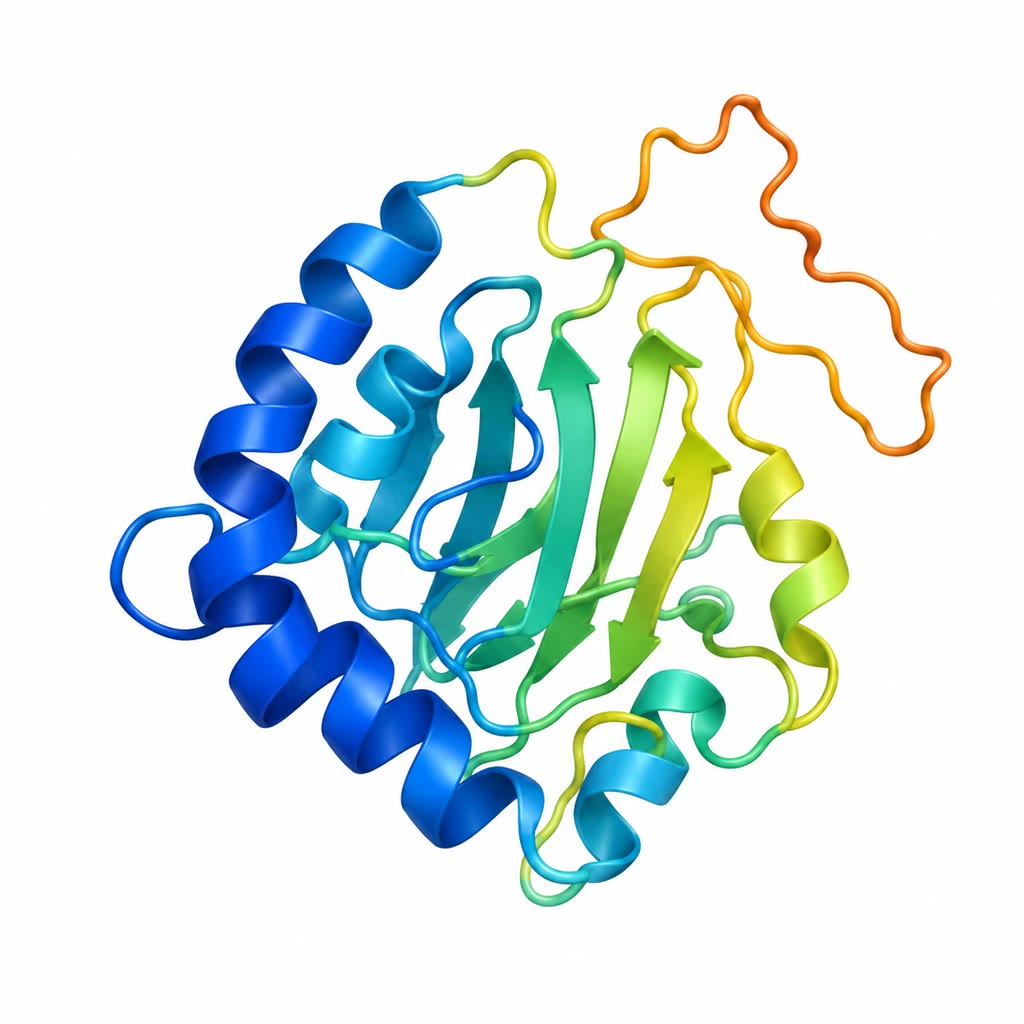
\includegraphics[width=0.36\linewidth]{images/book5/ai/b5-05-alphafold.jpg}\hspace{0.04\linewidth}
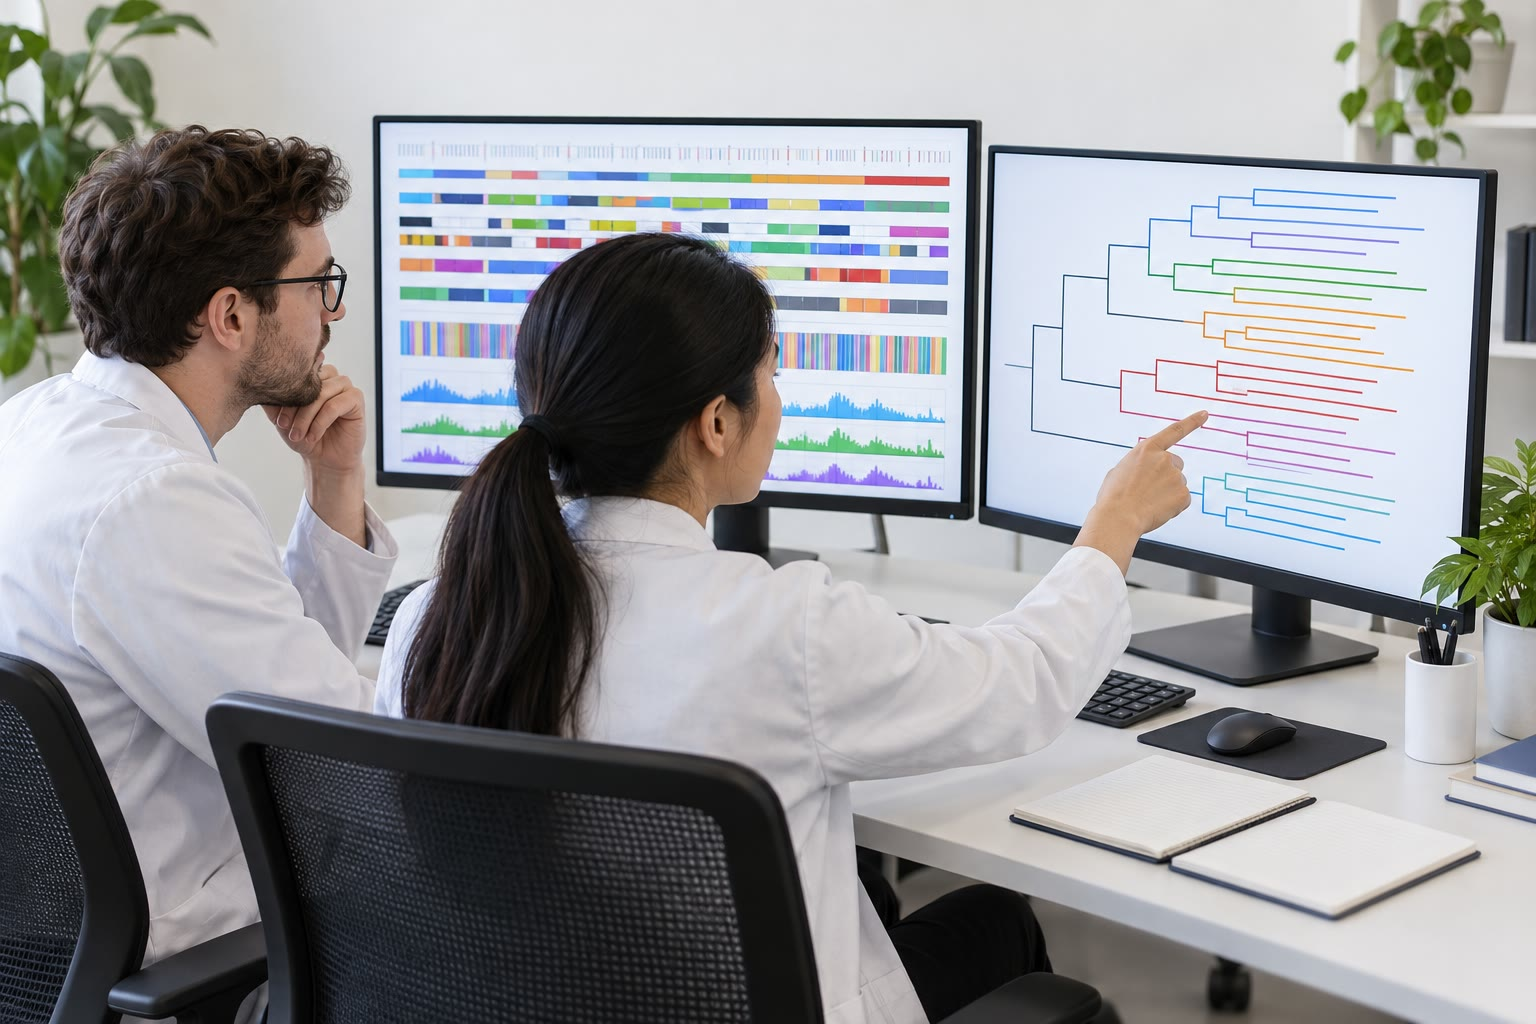
\includegraphics[width=0.54\linewidth]{images/book5/ai/b5-05-bioinformatics-lab.jpg}

{\small 左：预测的蛋白质结构，按模型的置信度着色，由高（蓝色）
到低（橙色），低置信度处为一段无序环区。
右：一间生物信息学办公室——
屏幕上是基因组浏览器和系统树，看不到湿实验台。}
\end{omfigure}

\begin{remark}[推断的局限]\label{rem:b3:bioinformatics:limits}
数据库中的大多数功能\omterm{def:b3:genomics:assembly}{注释}从未经过检验，它们是从同源序列转移而来的，
而该同源序列的\omterm{def:b3:genomics:assembly}{注释}本身又是经转移得到的。
错误会层层传递并不断放大，一条错误的\omterm{def:b3:genomics:assembly}{注释}若出现在连接度很高的蛋白质上，
就可能感染整个家族。补救办法即上文所述：
区分直系同源与同源，阅读\omterm{def:b3:bioinformatics:alignment}{比对}结果，
寻找催化残基，并记住“假定蛋白”
是一个诚实的标签，大多数基因组中仍有约三分之一的基因
配得上这一标签。
\end{remark}

\section{练习}

\begin{exercise}[$\star$]\label{exo:b3:bioinformatics:1}
定义\omterm{def:b3:bioinformatics:alignment}{全局比对}与\omterm{def:b3:bioinformatics:alignment}{局部比对}，
并各举一个需用该方法的生物学情境。
\end{exercise}

\begin{exercise}[$\star$]\label{exo:b3:bioinformatics:2}
对 AGC 与 AAC，以匹配 $+1$、
错配 $-1$、空位 $-1$ 的方案填写 Needleman--Wunsch 表，并给出最优\omterm{def:b3:bioinformatics:alignment}{比对}及其得分。
\end{exercise}

\begin{exercise}[$\star$]\label{exo:b3:bioinformatics:3}
在 BLOSUM62 中，色氨酸与色氨酸的得分为 $+11$，亮氨酸与亮氨酸的得分为
$+4$。试由对数几率公式说明，为何较稀有残基的相同之处
所得的分值更高。
\end{exercise}

\begin{exercise}[$\star$]\label{exo:b3:bioinformatics:4}
什么是 E 值？一次检索返回了一个 $E = 3$ 的命中。
这个数字意味着什么，该命中是否为同源序列？
\end{exercise}

\begin{exercise}[$\star\star$]\label{exo:b3:bioinformatics:5}
以一条含 \num{400} 个残基的查询序列检索 $2\times 10^{11}$
个残基的数据库。计算\omterm{thm:b3:bioinformatics:evalue}{比特得分}为 $45$、$55$ 和
$65$ 的命中的 E 值。哪一\omterm{thm:b3:bioinformatics:evalue}{比特得分}给出 $E = 10^{-3}$？若查询序列长度改为
\num{40} 个残基，结果如何变化？
\end{exercise}

\begin{exercise}[$\star\star$]\label{exo:b3:bioinformatics:6}
计算一个\omterm{def:b3:bioinformatics:motif}{基序}的\omterm{def:b3:bioinformatics:motif}{信息量}，该\omterm{def:b3:bioinformatics:motif}{基序}的四个位置上碱基频率（A、C、G、T）
依次为 $(1,0,0,0)$、$(0.5,0,0.5,0)$、
$(0.25,0.25,0.25,0.25)$ 与 $(0.7,0.1,0.1,0.1)$。该\omterm{def:b3:bioinformatics:motif}{基序}在
\qty{4.6}{Mb} 的基因组中会有多少次偶然匹配？
\end{exercise}

\begin{exercise}[$\star\star$]\label{exo:b3:bioinformatics:7}
解释为何仿射\omterm{def:b3:bioinformatics:alignment}{空位罚分}比线性\omterm{def:b3:bioinformatics:alignment}{空位罚分}更符合实际，
以及为何开启空位的罚分过高或过低，
都会得到较差的\omterm{def:b3:bioinformatics:alignment}{比对}。
\end{exercise}

\begin{exercise}[$\star\star$]\label{exo:b3:bioinformatics:8}
用 \omterm{def:b3:bioinformatics:blast}{BLAST} 以一条人类蛋白质检索果蝇数据库，得到的最佳命中
为 $E = 10^{-30}$，覆盖查询序列的第 50--180 位残基。
该查询序列含 \num{600} 个残基。
果蝇蛋白质是否为人类蛋白质的\omterm{def:b3:genomics:comparative}{直系同源基因}？还应做何种进一步检验？
\end{exercise}

\begin{exercise}[$\star\star$]\label{exo:b3:bioinformatics:9}
为何谱方法能检出两两\omterm{def:b3:bioinformatics:alignment}{比对}所遗漏的同源序列？
试举一个列模式的例子，它能被谱捕捉到，
而单条序列则无法体现。
\end{exercise}

\begin{exercise}[$\star\star\star$]\label{exo:b3:bioinformatics:10}
证明：在\omterm{prop:b3:bioinformatics:logodds}{期望得分}为正的打分方案下，两条长随机序列的
史密斯--Waterman \omterm{def:b3:bioinformatics:alignment}{局部比对}得分
随序列长度线性增长，并解释这为何使 E 值理论失效。
这一结论对于
采用匹配 $+1$ 与错配 $-1$ 的 DNA \omterm{def:b3:bioinformatics:alignment}{比对}，在 GC 含量为 \qty{60}{\%} 时意味着什么？
\end{exercise}

\begin{exercise}[$\star\star\star$]\label{exo:b3:bioinformatics:11}
Needleman--Wunsch 表需要 $mn$ 个存储单元。若对两条
长均为 \qty{100}{Mb} 的染色体进行\omterm{def:b3:bioinformatics:alignment}{比对}，所需存储单元即为 $10^{16}$。
描述两种让基因组\omterm{def:b3:bioinformatics:alignment}{比对}工具避开这一开销的思路（\omterm{def:b3:bioinformatics:blast}{种子}与链接；带状化），
并说明各自牺牲了什么。
\end{exercise}

\begin{exercise}[$\star\star\star$]\label{exo:b3:bioinformatics:12}
用于细菌基因查找的 HMM 具有三个密码子位置及非编码 DNA 的状态，
试解释该模型如何区分编码与非编码序列，
在完全不利用终止密码子信息的情况下（考虑密码子的使用偏好），
并说明为何同样的方法
在人类基因组中要困难得多。
\end{exercise}

\section{问题：来自深海的序列}

\begin{problem}[{周末问题——一条未知蛋白质经手工比对，
与数据库检索并计算其显著性，以比特衡量其调节基序，
并以随机开放阅读框的统计规律检验其基因，
最终归结于最佳命中的 E 值、
一个位点所需的比特数，以及阅读框须达到的长度，
方可采信}]
\label{pb:b3:bioinformatics:1}
数据：来自深海环节动物的一条 \num{300} 个残基的蛋白质。蛋白质数据库含
$1.2\times 10^{11}$ 个残基。该蠕虫的基因组为
\qty{1.6}{Gb}，GC 含量为 \qty{38}{\%}。手工\omterm{def:b3:bioinformatics:alignment}{比对}的打分方案：匹配 $+1$、
错配 $-1$、空位 $-1$。最佳 \omterm{def:b3:bioinformatics:blast}{BLAST} 命中的\omterm{thm:b3:bioinformatics:evalue}{比特得分}为 $92$，第十个命中的为
$38$。

\medskip
\noindent\textbf{第一部分——手工计算。}
\begin{enumerate}
  \item 用 Needleman--Wunsch 递推式\omterm{def:b3:bioinformatics:alignment}{比对}肽段 KQT 与 KAQT，
        写出计算表，给出最优\omterm{def:b3:bioinformatics:alignment}{比对}
        及其得分。
  \item 用\omterm{thm:b3:bioinformatics:nw}{史密斯–沃特曼}（局部）方法对 GATCAT 与 ACAT 重新\omterm{def:b3:bioinformatics:alignment}{比对}：
        求出最佳\omterm{def:b3:bioinformatics:alignment}{局部比对}及其得分。
  \item 用\omterm{def:b3:bioinformatics:alignment}{全局比对}方法将
        \num{300} 个残基的蛋白质与 \num{450} 个残基的蛋白质\omterm{def:b3:bioinformatics:alignment}{比对}，
        需要多少次细胞更新？与整个数据库\omterm{def:b3:bioinformatics:alignment}{比对}呢？
  \item 若计算机每秒执行 $10^{9}$ 次更新，
        则问题 3 中与整个数据库的\omterm{def:b3:bioinformatics:alignment}{比对}需要多长时间？
        为何改用 \omterm{def:b3:bioinformatics:blast}{BLAST}？
  \item BLOSUM62 中，丙氨酸的同一性得分为 $+4$（$p_{A} =
        0.074$），色氨酸的同一性得分为 $+11$（$p_{W} = 0.013$）。
        取 $\lambda = 0.347$（半比特单位），
        分别计算目标频率 $q_{AA}$ 与 $q_{WW}$，以及各自的比值 $q/p^{2}$，
        并加以解释。
  \item 两个蛋白质在 $250$ 个残基上的同一性为 \qty{24}{\%}。
        说明在此情形下仅凭同一性为何无法判定同源性，
        并指出需要什么才能判定。
\end{enumerate}

\medskip
\noindent\textbf{第二部分——检索。}
\begin{enumerate}[resume]
  \item 计算查询序列对数据库的 $mn$，以及
        $\log_{2}(mn)$。
  \item 计算最佳命中（$S' = 92$）的 E 值，以及
        第十个命中（$S' = 38$）的 E 值。
  \item 在本次检索中，$E = 10^{-3}$ 对应多少\omterm{thm:b3:bioinformatics:evalue}{比特得分}？
        $E = 1$ 呢？
  \item 当数据库增长到
        $1.2\times 10^{12}$ 个残基时，同一最佳命中仍被找到。其 E 值为多少？
  \item 第十个命中将查询序列的第 200--260 位残基与之\omterm{def:b3:bioinformatics:alignment}{比对}，
        在 $60$ 个残基上的同一性为 \qty{40}{\%}，利用 E 值
        判断它是否为同源的证据，
        并说明谱检索还能提供什么。
  \item 最佳命中是一个人类激酶，
        \omterm{def:b3:bioinformatics:alignment}{比对}范围为第 10--290 位残基。其在蠕虫蛋白质组中的最佳命中
        即为该查询序列。这一互为最佳命中的检验能说明什么，又不能说明什么？
\end{enumerate}

\medskip
\noindent\textbf{第三部分——\omterm{def:b3:bioinformatics:motif}{基序}。}
\begin{enumerate}[resume]
  \item 基因上游有一个候选转录因子位点，
        长 8 个位置，各位置的\omterm{def:b3:bioinformatics:motif}{信息量}依次为
        $2, 2, 1.6, 2, 0.8, 1.2, 0.4, 0.3$ 比特。求总的 $R$？
  \item 该\omterm{def:b3:bioinformatics:motif}{基序}在 \qty{1.6}{Gb} 基因组中有多少次偶然匹配
        （两条链，共 $3.2\times 10^{9}$
        个位置）？
  \item 该因子调控约 $200$ 个基因。
        仅凭一个\omterm{def:b3:bioinformatics:motif}{基序}，要在此基因组中确定 $200$ 个位点，需要多少比特？
  \item 若与之相邻的第二个\omterm{def:b3:bioinformatics:motif}{基序}为
        $8$ 比特，且两者须在固定间距内共现，
        它能补足多少不足部分？
  \item 某位置的频率依次为 $(0.5, 0.5, 0, 0)$，对应 (A, C, G,
        T)：计算其熵与\omterm{def:b3:bioinformatics:motif}{信息量}。
  \item 利用信息论论证，说明为何细菌转录因子
        的位点通常比真核生物的更长，
        且更为保守。
\end{enumerate}

\medskip
\noindent\textbf{第四部分——基因本身。}
\begin{enumerate}[resume]
  \item 在碱基组成均匀的随机 DNA 中，
        一个密码子为终止密码子的概率是多少？期望的
        密码子数（在终止密码子出现之前）是多少
        （几何分布）？
  \item 蠕虫基因组的 GC 含量为 \qty{38}{\%}，
        用实际碱基频率重新计算随机密码子为终止密码子
        （TAA、TAG、TGA）的概率，以及期望的阅读框长度。
        低 GC 含量对基因查找有何影响？
  \item 随机开放阅读框长度至少为
        $100$ 个密码子的概率是多少？至少为 $300$ 个密码子呢？
  \item 在 \qty{1.6}{Gb} 基因组中，两条链上的六个阅读框约有
        $3.2\times 10^{9}$ 个密码子起始位点。期望有多少个
        至少含 $100$ 个密码子的随机开放阅读框？
        至少含 $300$ 个密码子的呢？
  \item 说明为何“长于 $100$ 个密码子的开放阅读框”
        在细菌中可用作基因查找方法，而在该基因组中则不然，
        并指出真核生物的基因查找改用什么方法。
  \item 蠕虫基因有六个外显子，平均长度为 \qty{150}{bp}。说明
        RNA 测序读段如何解析
        仅凭基因组序列无法确定的外显子结构。
  \item 总结：最佳命中的 E 值（问题~8）、
        确定 $200$ 个位点所需的比特数（问题~15），以及
        基因组中长 $300$ 个密码子的随机阅读框的期望数
        （问题~22）。
\end{enumerate}
\end{problem}
